\chapter{Machine learning algorithms comparison} \label{chap:methods}

Before going further and analysing neural networks, we will take a deeper look at classical machine learning algorithms, in particular Random Forests and Support Vector Machine (SVM) in the context of anomaly detection in the CPS presented in chapter \ref{chap:intro}. However this was done before in \cite{borges_hink_machine_2014-1} using the black-box model only. In their approach they used Weka \cite{witten_appendix_2017} in order to find the most performant algorithm among 7 they have chosen (OneR, NNge, Random Forests, Naïve Bayes, SVM, JRipper, Adaboost). Weka is an open source machine learning software. One of its advantages is a graphical interface, that is easy to use. 

The following sections show an attempt to reproduce the the results provided in \cite{borges_hink_machine_2014-1}, first using Weka, then scikit-learn \cite{pedregosa_scikit-learn_2011} to model the machine learning algorithms. The choice of scikit-learn was based on its versatility and configurability, which will be an asset in further modifications of the used algorithms.

\section{Weka} \label{sec:weka_in_chap:methods}

\begin{figure}[H]
    \centering
    \begin{subfigure}[t]{0.5\textwidth}
        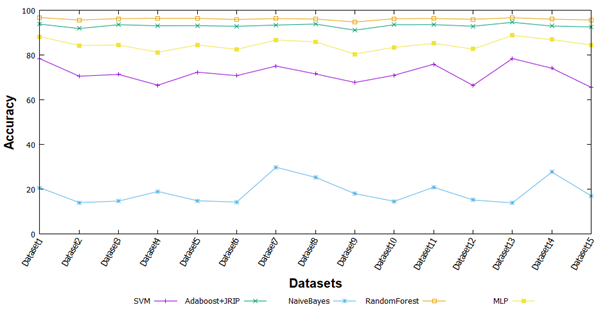
\includegraphics[width=\linewidth]{images/weka_accuracy.png}
        \caption{Our attempt}
    \end{subfigure}%
    \begin{subfigure}[t]{0.5\textwidth}
        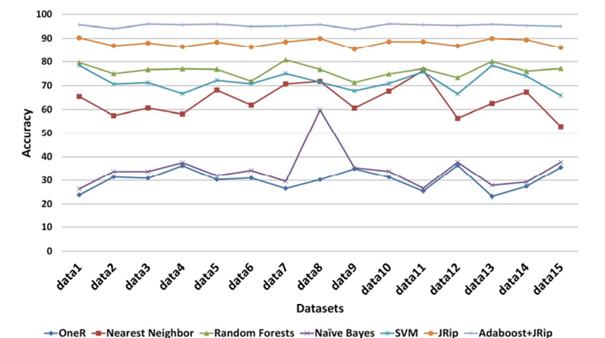
\includegraphics[width=\linewidth]{images/weka_accuracy_cite.png}
        \caption{Original results \cite{borges_hink_machine_2014-1}}
    \end{subfigure}
    \caption{Accuracy}
\end{figure}

\begin{figure}[H]
    \centering
    \begin{subfigure}[t]{0.5\textwidth}
        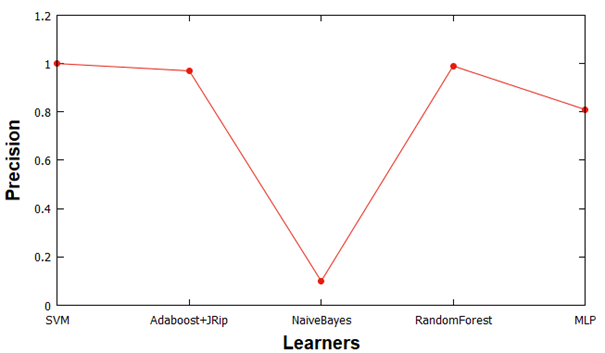
\includegraphics[width=\linewidth]{images/weka_precision.png}
        \caption{Our attempt}
    \end{subfigure}%
    \begin{subfigure}[t]{0.5\textwidth}
        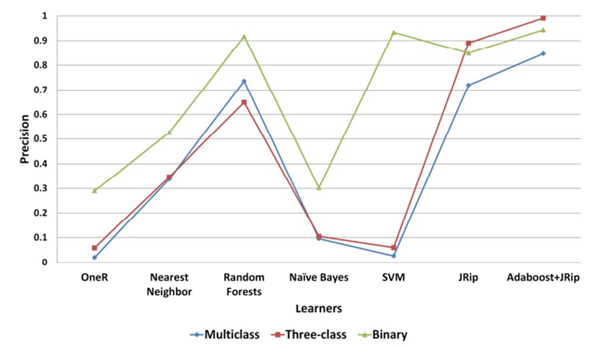
\includegraphics[width=\linewidth]{images/weka_precision_cite.png}
        \caption{Original results \cite{borges_hink_machine_2014-1}}
    \end{subfigure}
    \caption{Precision}
\end{figure}

\begin{figure}[H]
    \centering
    \begin{subfigure}[t]{0.5\textwidth}
        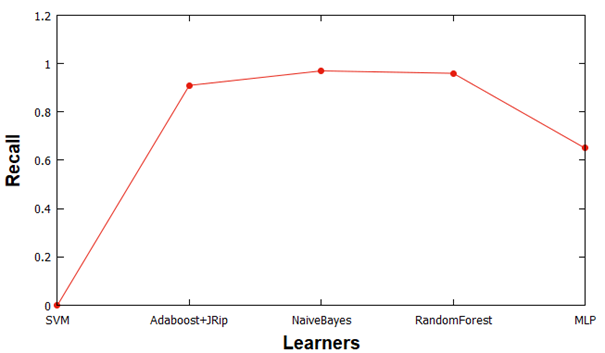
\includegraphics[width=\linewidth]{images/weka_recall.png}
        \caption{Our attempt}
    \end{subfigure}%
    \begin{subfigure}[t]{0.5\textwidth}
        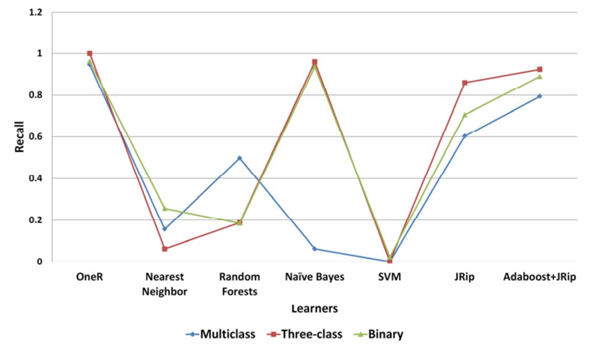
\includegraphics[width=\linewidth]{images/weka_recall_cite.png}
        \caption{Original results \cite{borges_hink_machine_2014-1}}
    \end{subfigure}
    \caption{Recall}
\end{figure}

\begin{figure}[H]
    \centering
    \begin{subfigure}[t]{0.5\textwidth}
        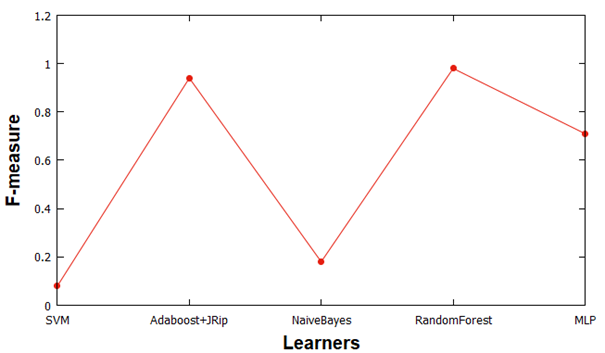
\includegraphics[width=\linewidth]{images/weka_f1.png}
        \caption{Our attempt}
    \end{subfigure}%
    \begin{subfigure}[t]{0.5\textwidth}
        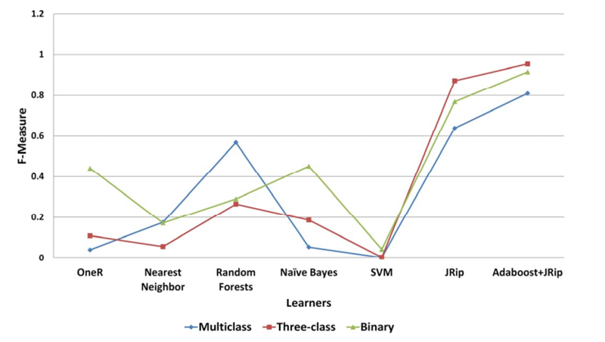
\includegraphics[width=\linewidth]{images/weka_f1_cite.png}
        \caption{Original results \cite{borges_hink_machine_2014-1}}
    \end{subfigure}
    \caption{F-measure}
\end{figure}

\section{scikit-learn} \label{sec:scikit_in_chap:methods}

\begin{figure}[H]
    \centering
    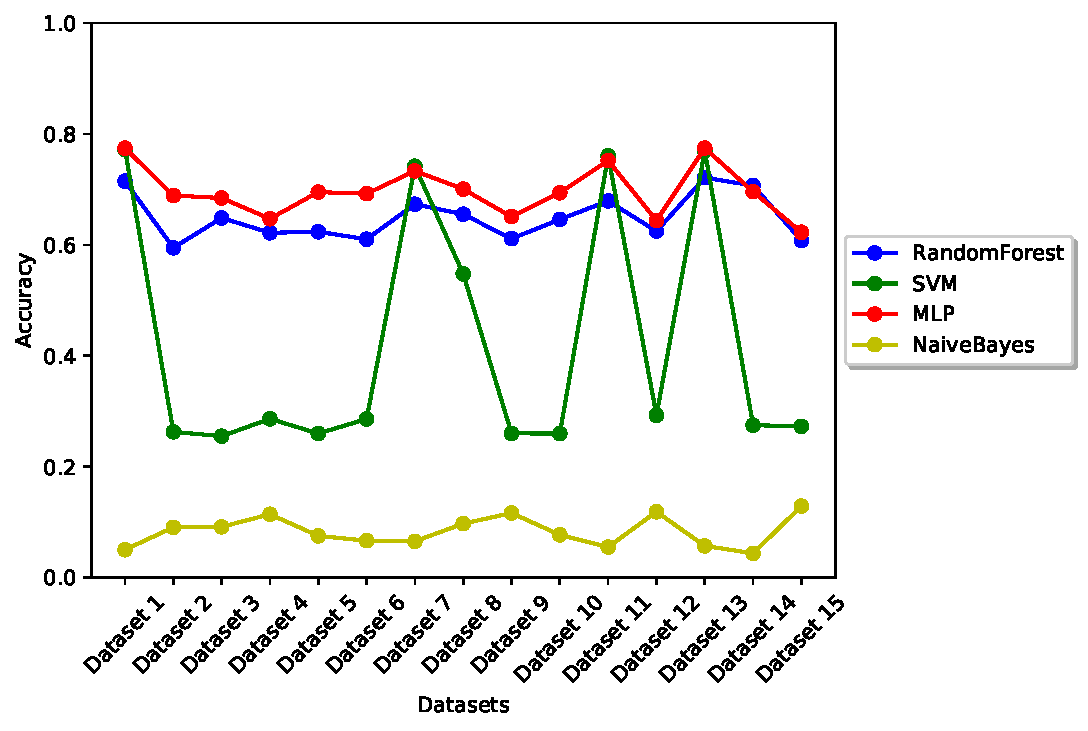
\includegraphics[page=1, width=100mm]{images/results_scikit.pdf}
    \caption{Accuracy}
    \label{fig_scikit_accuracy}
\end{figure}

\begin{figure}[H]
    \centering
    \includegraphics[page=2, width=100mm]{images/results_scikit.pdf}
    \caption{F-measure}
    \label{fig_scikit_f1}
\end{figure}

\begin{figure}[H]
    \centering
    \includegraphics[page=3, width=100mm]{images/results_scikit.pdf}
    \caption{Precision}
    \label{fig_scikit_prec}
\end{figure}

\begin{figure}[H]
    \centering
    \includegraphics[page=4, width=100mm]{images/results_scikit.pdf}
    \caption{Recall}
    \label{fig_scikit_recall}
\end{figure}

\subsection{Random Forests}

\begin{figure}[H]
    \centering
    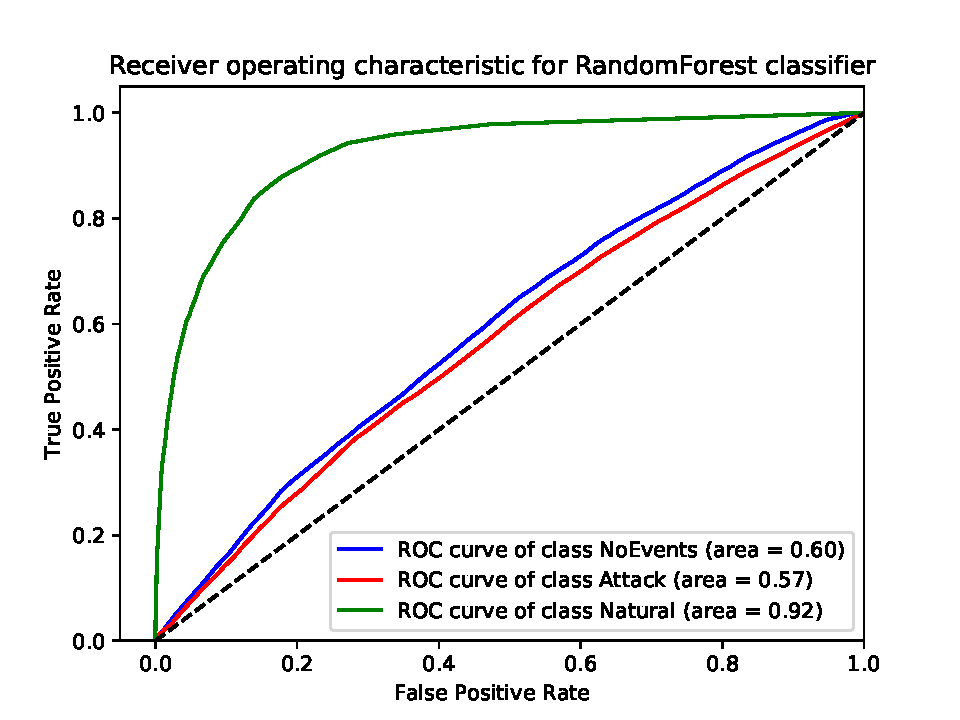
\includegraphics[page=1, width=100mm]{images/results_scikit/RandomForest}
    \caption{ROC Curve for Random Forests}
    \label{fig_scikit_RF_ROC}
\end{figure}

\begin{figure}[H]
    \centering
    \includegraphics[page=2, width=100mm, trim= 0 50 0 100, clip]{images/results_scikit/RandomForest}
    \caption{Confusion Matrix for Random Forests}
    \label{fig_scikit_CM_ROC}
\end{figure}

\subsection{SVM}

\begin{figure}[H]
    \centering
    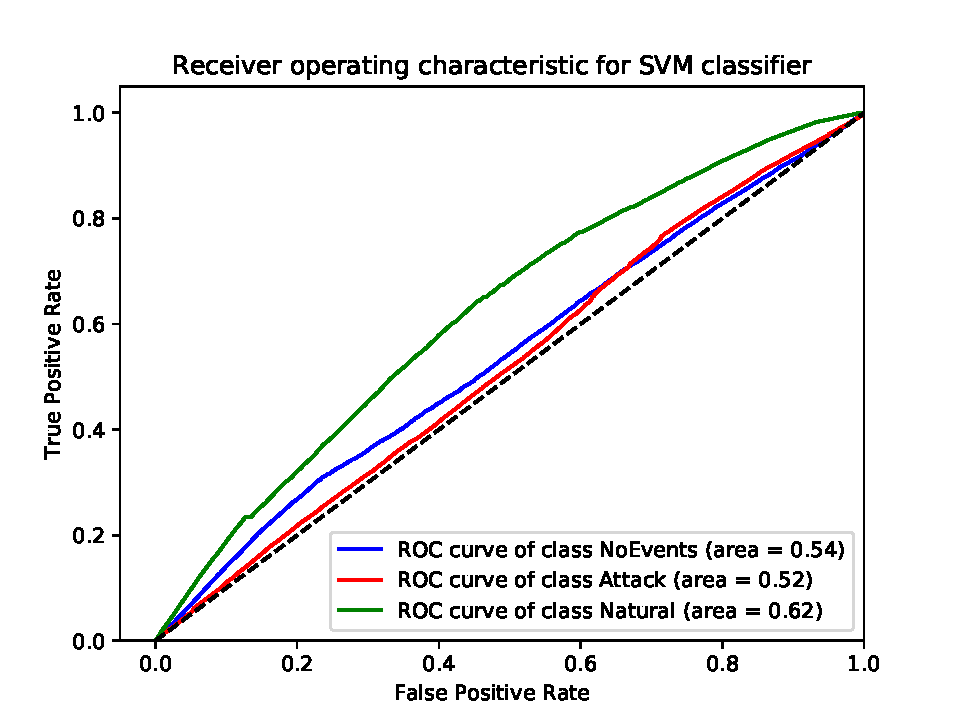
\includegraphics[page=1, width=100mm]{images/results_scikit/SVM}
    \caption{ROC Curve for SVM}
    \label{fig_scikit_SVM_ROC}
\end{figure}

\begin{figure}[H]
    \centering
    \includegraphics[page=2, width=100mm, trim= 0 50 0 100, clip]{images/results_scikit/SVM}
    \caption{Confusion Matrix for SVM}
    \label{fig_scikit_SVM_ROC}
\end{figure}

\subsection{Naïve Bayes}

\begin{figure}[H]
    \centering
    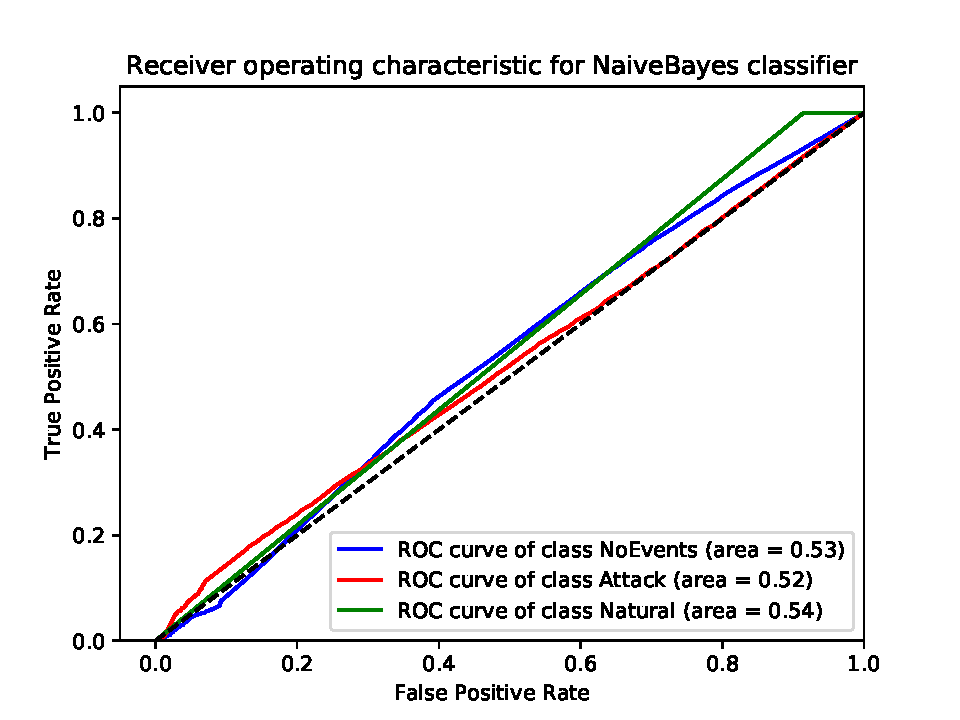
\includegraphics[page=1, width=100mm]{images/results_scikit/NaiveBayes}
    \caption{ROC Curve for Naïve Bayes}
    \label{fig_scikit_NB_ROC}
\end{figure}

\begin{figure}[H]
    \centering
    \includegraphics[page=2, width=100mm, trim= 0 50 0 100, clip]{images/results_scikit/NaiveBayes}
    \caption{Confusion Matrix for Naïve Bayes}
    \label{fig_scikit_NB_ROC}
\end{figure}

\subsection{MLP}

\begin{figure}[H]
    \centering
    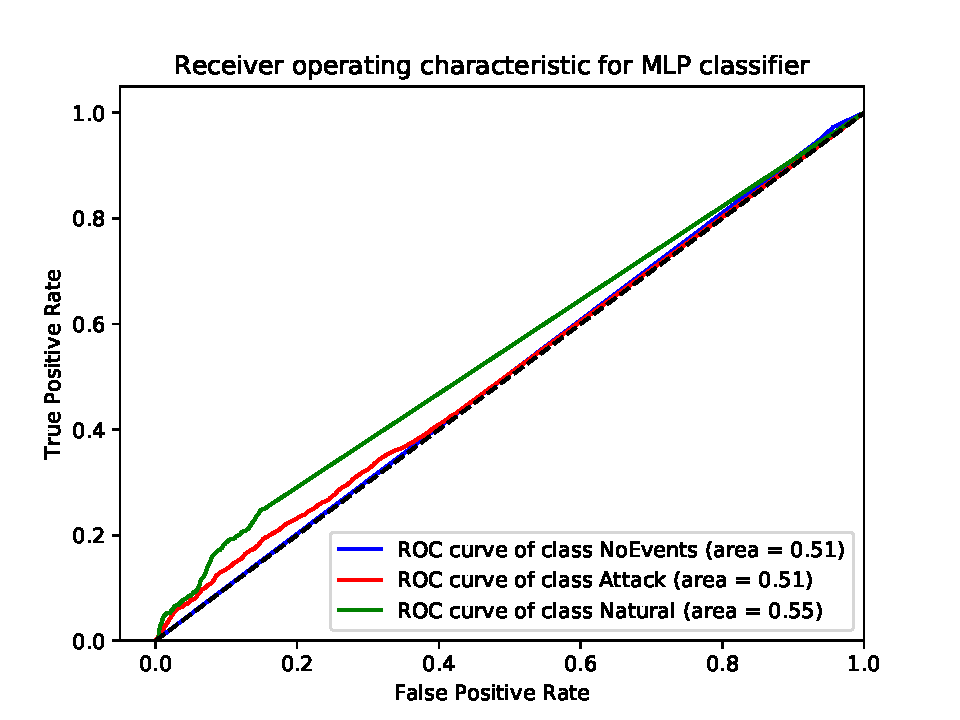
\includegraphics[page=1, width=100mm]{images/results_scikit/MLP}
    \caption{ROC Curve for MLP}
    \label{fig_scikit_MLP_ROC}
\end{figure}

\begin{figure}[H]
    \centering
    \includegraphics[page=2, width=100mm, trim= 0 50 0 100, clip]{images/results_scikit/MLP}
    \caption{Confusion Matrix for MLP}
    \label{fig_scikit_MLP_ROC}
\end{figure}



